\documentclass[journal,12pt,twocolumn]{IEEEtran}
\usepackage{setspace}
\usepackage{gensymb}
\usepackage{caption}
%\usepackage{multirow}
%\usepackage{multicolumn}
%\usepackage{subcaption}
%\doublespacing
\singlespacing
\usepackage{csvsimple}
\usepackage{amsmath}
\usepackage{multicol}
%\usepackage{enumerate}
\usepackage{amssymb}
%\usepackage{graphicx}
\usepackage{newfloat}
%\usepackage{syntax}
\usepackage{listings}
\usepackage{color}
\usepackage{tikz}
\usetikzlibrary{shapes,arrows}



%\usepackage{graphicx}
%\usepackage{amssymb}
%\usepackage{relsize}
%\usepackage[cmex10]{amsmath}
%\usepackage{mathtools}
%\usepackage{amsthm}
%\interdisplaylinepenalty=2500
%\savesymbol{iint}
%\usepackage{txfonts}
%\restoresymbol{TXF}{iint}
%\usepackage{wasysym}
\usepackage{amsthm}
\usepackage{mathrsfs}
\usepackage{txfonts}
\usepackage{stfloats}
\usepackage{cite}
\usepackage{cases}
\usepackage{mathtools}
\usepackage{caption}
\usepackage{enumerate}	
\usepackage{enumitem}
\usepackage{amsmath}
%\usepackage{xtab}
\usepackage{longtable}
\usepackage{multirow}
%\usepackage{algorithm}
%\usepackage{algpseudocode}
\usepackage{enumitem}
\usepackage{mathtools}
\usepackage{hyperref}
%\usepackage[framemethod=tikz]{mdframed}
\usepackage{listings}
    %\usepackage[latin1]{inputenc}                                 %%
    \usepackage{color}                                            %%
    \usepackage{array}                                            %%
    \usepackage{longtable}                                        %%
    \usepackage{calc}                                             %%
    \usepackage{multirow}                                         %%
    \usepackage{hhline}                                           %%
    \usepackage{ifthen}                                           %%
  %optionally (for landscape tables embedded in another document): %%
    \usepackage{lscape}     


\usepackage{url}
\def\UrlBreaks{\do\/\do-}


%\usepackage{stmaryrd}


%\usepackage{wasysym}
%\newcounter{MYtempeqncnt}
\DeclareMathOperator*{\Res}{Res}
%\renewcommand{\baselinestretch}{2}
\renewcommand\thesection{\arabic{section}}
\renewcommand\thesubsection{\thesection.\arabic{subsection}}
\renewcommand\thesubsubsection{\thesubsection.\arabic{subsubsection}}

\renewcommand\thesectiondis{\arabic{section}}
\renewcommand\thesubsectiondis{\thesectiondis.\arabic{subsection}}
\renewcommand\thesubsubsectiondis{\thesubsectiondis.\arabic{subsubsection}}

% correct bad hyphenation here
\hyphenation{op-tical net-works semi-conduc-tor}

%\lstset{
%language=C,
%frame=single, 
%breaklines=true
%}

%\lstset{
	%%basicstyle=\small\ttfamily\bfseries,
	%%numberstyle=\small\ttfamily,
	%language=Octave,
	%backgroundcolor=\color{white},
	%%frame=single,
	%%keywordstyle=\bfseries,
	%%breaklines=true,
	%%showstringspaces=false,
	%%xleftmargin=-10mm,
	%%aboveskip=-1mm,
	%%belowskip=0mm
%}

%\surroundwithmdframed[width=\columnwidth]{lstlisting}
\def\inputGnumericTable{}                                 %%
\lstset{
%language=C,
frame=single, 
breaklines=true,
columns=fullflexible
}
 

\begin{document}
%
\tikzstyle{block} = [rectangle, draw,
    text width=3em, text centered, minimum height=3em]
\tikzstyle{sum} = [draw, circle, node distance=3cm]
\tikzstyle{input} = [coordinate]
\tikzstyle{output} = [coordinate]
\tikzstyle{pinstyle} = [pin edge={to-,thin,black}]
\providecommand{\e}[1]{\ensuremath{E\left(#1\right)}}
\providecommand{\es}[1]{\ensuremath{E\left[#1\right]}}
\theoremstyle{definition}
\newtheorem{theorem}{Theorem}[section]
\newtheorem{problem}{Problem}
\newtheorem{proposition}{Proposition}[section]
\newtheorem{lemma}{Lemma}[section]
\newtheorem{corollary}[theorem]{Corollary}
\newtheorem{example}{Example}[section]
\newtheorem{definition}{Definition}[section]
%\newtheorem{algorithm}{Algorithm}[section]
%\newtheorem{cor}{Corollary}
\newcommand{\BEQA}{\begin{eqnarray}}
\newcommand{\EEQA}{\end{eqnarray}}
\newcommand{\define}{\stackrel{\triangle}{=}}
\bibliographystyle{IEEEtran}
%\bibliographystyle{ieeetr}
\providecommand{\nCr}[2]{\,^{#1}C_{#2}} % nCr
\providecommand{\nPr}[2]{\,^{#1}P_{#2}} % nPr
\providecommand{\mbf}{\mathbf}
\providecommand{\pr}[1]{\ensuremath{\Pr\left(#1\right)}}
\providecommand{\qfunc}[1]{\ensuremath{Q\left(#1\right)}}
\providecommand{\sbrak}[1]{\ensuremath{{}\left[#1\right]}}
\providecommand{\lsbrak}[1]{\ensuremath{{}\left[#1\right.}}
\providecommand{\rsbrak}[1]{\ensuremath{{}\left.#1\right]}}
\providecommand{\brak}[1]{\ensuremath{\left(#1\right)}}
\providecommand{\lbrak}[1]{\ensuremath{\left(#1\right.}}
\providecommand{\rbrak}[1]{\ensuremath{\left.#1\right)}}
\providecommand{\cbrak}[1]{\ensuremath{\left\{#1\right\}}}
\providecommand{\lcbrak}[1]{\ensuremath{\left\{#1\right.}}
\providecommand{\rcbrak}[1]{\ensuremath{\left.#1\right\}}}
\theoremstyle{remark}
\newtheorem{rem}{Remark}
\newcommand{\sgn}{\mathop{\mathrm{sgn}}}
% \providecommand{\abs}[1]{\left\vert#1\right\vert}
% \providecommand{\res}[1]{\Res\displaylimits_{#1}} 
% \providecommand{\norm}[1]{\left\Vert#1\right\Vert}
% \providecommand{\mtx}[1]{\mathbf{#1}}
% \providecommand{\mean}[1]{E\left[ #1 \right]}
\providecommand{\fourier}{\overset{\mathcal{F}}{ \rightleftharpoons}}
%\providecommand{\hilbert}{\overset{\mathcal{H}}{ \rightleftharpoons}}
\providecommand{\system}{\overset{\mathcal{H}}{ \longleftrightarrow}}
	%\newcommand{\solution}[2]{\textbf{Solution:}{#1}}
\newcommand{\solution}{\noindent \textbf{Solution: }}
\newcommand{\myvec}[1]{\ensuremath{\begin{pmatrix}#1\end{pmatrix}}}
\providecommand{\dec}[2]{\ensuremath{\overset{#1}{\underset{#2}{\gtrless}}}}
\DeclarePairedDelimiter{\ceil}{\lceil}{\rceil}
%\numberwithin{equation}{section}
%\numberwithin{problem}{subsection}
%\numberwithin{definition}{subsection}
\makeatletter
\@addtoreset{figure}{section}
\makeatother
\let\StandardTheFigure\thefigure
%\renewcommand{\thefigure}{\theproblem.\arabic{figure}}
\renewcommand{\thefigure}{\thesection}
%\numberwithin{figure}{subsection}
%\numberwithin{equation}{subsection}
%\numberwithin{equation}{section}
%\numberwithin{equation}{problem}
%\numberwithin{problem}{subsection}
\numberwithin{problem}{section}
%%\numberwithin{definition}{subsection}
%\makeatletter
%\@addtoreset{figure}{problem}
%\makeatother
\makeatletter
\@addtoreset{table}{section}
\makeatother
\let\StandardTheFigure\thefigure
\let\StandardTheTable\thetable
\let\vec\mathbf
\numberwithin{equation}{section}
\vspace{3cm}
\title{%Convex Optimization in Python
	{
	Assignment
	}
}
%\title{
%	\logo{Matrix Analysis through Octave}{\begin{center}\includegraphics[scale=.24]{tlc}\end{center}}{}{HAMDSP}
%}
% paper title
% can use linebreaks \\ within to get better formatting as desired
%\title{Matrix Analysis through Octave}
%
%
% author names and IEEE memberships
% note positions of commas and nonbreaking spaces ( ~ ) LaTeX will not break
% a structure at a ~ so this keeps an author's name from being broken across
% two lines.
% use \thanks{} to gain access to the first footnote area
% a separate \thanks must be used for each paragraph as LaTeX2e's \thanks
% was not built to handle multiple paragraphs
%
\author{R Bhargava Ram \\ CS21BTECH11052}
% note the % following the last \IEEEmembership and also \thanks - 
% these prevent an unwanted space from occurring between the last author name
% and the end of the author line. i.e., if you had this:
% 
% \author{....lastname \thanks{...} \thanks{...} }
%                     ^------------^------------^----Do not want these spaces!
%
% a space would be appended to the last name and could cause every name on that
% line to be shifted left slightly. This is one of those "LaTeX things". For
% instance, "\textbf{A} \textbf{B}" will typeset as "A B" not "AB". To get
% "AB" then you have to do: "\textbf{A}\textbf{B}"
% \thanks is no different in this regard, so shield the last } of each \thanks
% that ends a line with a % and do not let a space in before the next \thanks.
% Spaces after \IEEEmembership other than the last one are OK (and needed) as
% you are supposed to have spaces between the names. For what it is worth,
% this is a minor point as most people would not even notice if the said evil
% space somehow managed to creep in.
% The paper headers
%\markboth{Journal of \LaTeX\ Class Files,~Vol.~6, No.~1, January~2007}%
%{Shell \MakeLowercase{\textit{et al.}}: Bare Demo of IEEEtran.cls for Journals}
% The only time the second header will appear is for the odd numbered pages
% after the title page when using the twoside option.
% 
% *** Note that you probably will NOT want to include the author's ***
% *** name in the headers of peer review papers.                   ***
% You can use \ifCLASSOPTIONpeerreview for conditional compilation here if
% you desire.
% If you want to put a publisher's ID mark on the page you can do it like
% this:
%\IEEEpubid{0000--0000/00\$00.00~\copyright~2007 IEEE}
% Remember, if you use this you must call \IEEEpubidadjcol in the second
% column for its text to clear the IEEEpubid mark.
% make the title area
\maketitle
\tableofcontents
\bigskip
\renewcommand{\thefigure}{\theenumi}
\renewcommand{\thetable}{\theenumi}
\begin{abstract}
This manual provides solutions to the Assignment on Random Numbers
\end{abstract}
%template ends here
\section{Uniform Random Numbers}
Let $U$ be a uniform random variable between 0 and 1.
\begin{enumerate}[label=\thesection.\arabic*
,ref=\thesection.\theenumi]

%%%%%%%%%%%%%%%%%%%%%%%%%%%%%%%%%%%%%%%%
\item Generate $10^6$ samples of $U$ using a C program and save into a file called uni.dat .
\\
\solution Download the following files and execute the  C program.
\begin{lstlisting}
https://github.com/bhargav0383/AI1110-Assignments/blob/main/RandomNumbers/codes/1.1.c
https://github.com/bhargav0383/AI1110-Assignments/blob/main/RandomNumbers/codes/functions.h
\end{lstlisting}
Execute the above C program files using the following commands
\begin{lstlisting}
$ gcc 1.1.c
$ ./a.out
\end{lstlisting}

%%%%%%%%%%%%%%%%%%%%%%%%%%%%%%%%%%%%%%
\item
Load the uni.dat file into python and plot the empirical CDF of $U$ using the samples in uni.dat. The CDF is defined as
\begin{align}
F_{U}(x) = \pr{U \le x}
\end{align}
\\
\solution  The python code for the plot in Fig. \ref{fig:1.2} is given below,
\begin{lstlisting}
https://github.com/bhargav0383/AI1110-Assignments/blob/main/RandomNumbers/codes/1.2CDF.py
\end{lstlisting}
Download the above file and execute the command below to produce Fig.\ref{fig:1.2}
\begin{lstlisting}
$ python3 1.2CDF.py
\end{lstlisting}
\begin{figure}[!h]
\centering
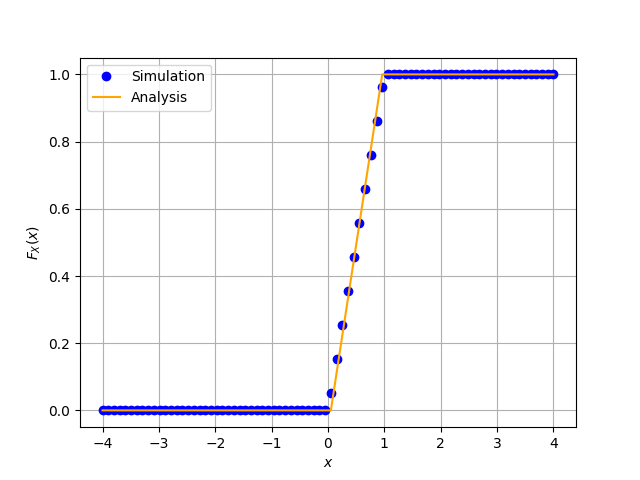
\includegraphics[width=\columnwidth]{./figs/1.2CDF.png}
\caption{The CDF of $U$}
\label{fig:1.2}
\end{figure}
%

%%%%%%%%%%%%%%%%%%%%%%%%%%%%%%%%%%%%%%%%
\item
Find a  theoretical expression for $F_{U}(x)$.\\
\solution Given $U$ is a uniform Random Variable between 0 and 1,
\begin{align}
F_U(x) = \pr{U \leq x} = \int_{-\infty}^{x}p_U(u)du
\end{align}
We have three parts:
		\begin{enumerate}[label=\roman*)]
			\item For $x < 0$; $p_X(x) = 0$, So $F_U(x) = 0$.
			\item For $0 \leq x < 1$;
				\begin{align}
					F_U(x) = \int_{0}^{x}(1)du = x
				\end{align}
			\item For $x \geq 1$; CDF is 1 as all the random numbers are between 0 and 1.
		\end{enumerate}
Therefore,
		\begin{align}
			F_U(x) = 
			\begin{cases}
				0 & x < 0 \\
				x & 0 \leq x < 1 \\
				1 & x \geq 1
			\end{cases}
		\end{align}
		
%%%%%%%%%%%%%%%%%%%%%%%%%%%%%%%%%%%%%%%%%%%%%%%%%
\item
The mean of $U$ is defined as
%
\begin{equation}
E\sbrak{U} = \frac{1}{N}\sum_{i=1}^{N}U_i
\end{equation}
%
and its variance as
%
\begin{equation}
\text{var}\sbrak{U} = E\sbrak{U- E\sbrak{U}}^2 
\end{equation}
Write a C program to  find the mean and variance of $U$. \\

\solution Download the following files and execute the  C program.
\begin{lstlisting}
https://github.com/bhargav0383/AI1110-Assignments/blob/main/RandomNumbers/codes/1.4.c
https://github.com/bhargav0383/AI1110-Assignments/blob/main/RandomNumbers/codes/functions.h
\end{lstlisting}
Execute the above C program files using the following commands
\begin{lstlisting}
$ gcc 1.4.c
$ ./a.out
\end{lstlisting}
The actual analysis values,
\begin{align}
    \text{Mean}&= 0.500007  \\
    \text{Variance} &=  0.083301
\end{align}
%%%%%%%%%%%%%%%%%%%%%%%%%%%%%%%%%%%%%%%%%%%%%%%%%%%%%%%%%%%%%
\item Verify your result theoretically given that
\end{enumerate}
%
\begin{equation}
E\sbrak{U^k} = \int_{-\infty}^{\infty}x^kdF_{U}(x)
\end{equation}
\solution 
W.K.T,
\begin{align}
    \text{var}\sbrak{U} &= E\sbrak{U^2}- E\sbrak{U}^2
\end{align}
Where $E\sbrak{U}$ is,
\begin{align}
   E\sbrak{U}&=\int_{-\infty}^{\infty}xdF_U(x)\\
             &=\int_{0}^{1}x\\
             &=\frac{1}{2} = 0.5
\end{align}
And $E\sbrak{U^2}$ is,
\begin{align}
    E\sbrak{U^2}&=\int_{-\infty}^{\infty}x^{2}dF_U(x)\\
                &=\int_{0}^{1}x^{2}dF_U(x)\\
                &=\frac{1}{3}\\
\end{align}
Hence finally,
\begin{align}
    \therefore \boxed{\text{var}\sbrak{U}=\frac{1}{12}=0.0833}
\end{align}
The theoretically calculated values are,
\begin{align}
    \text{Mean}&= 0.5  \\
    \text{Variance} &=  0.0833
\end{align}
These values matches with the actual analysis values from above,
\begin{align}
    \text{Mean}&= 0.500007  \\
    \text{Variance} &=  0.083301
\end{align}
Hence it verifies the result.
%%%%%%%%%%%%%%%%%%%%%%%%%%%%%%%%%%%%%%%%%%%%%%%%%%%%%%%%%%%%%%%%%
\section{Central Limit Theorem}
%
\begin{enumerate}[label=\thesection.\arabic*
,ref=\thesection.\theenumi]
%
\item
Generate $10^6$ samples of the random variable
%
\begin{equation}
X = \sum_{i=1}^{12}U_i -6
\end{equation}
%
using a C program, where $U_i, i = 1,2,\dots, 12$ are  a set of independent uniform random variables between 0 and 1 and save in a file called gau.dat\\
\solution Download the following files and execute the  C program.
\begin{lstlisting}
https://github.com/bhargav0383/AI1110-Assignments/blob/main/RandomNumbers/codes/2.1.c
https://github.com/bhargav0383/AI1110-Assignments/blob/main/RandomNumbers/codes/functions.h
\end{lstlisting}
Execute the above C program files using the following commands
\begin{lstlisting}
$ gcc 2.1.c
$ ./a.out
\end{lstlisting}

%%%%%%%%%%%%%%%%%%%%%%%%%%%%%%%%%%%%%%%%%%%%%%%%%
\item
Load gau.dat in python and plot the empirical CDF of $X$ using the samples in gau.dat. What properties does a CDF have?\\
\solution The CDF of $X$ is plotted in Fig. \ref{fig:2.2}\\
using the code below
\begin{lstlisting}
https://github.com/bhargav0383/AI1110-Assignments/blob/main/RandomNumbers/codes/2.2CDF.py
\end{lstlisting}
\begin{figure}[!h]
\centering
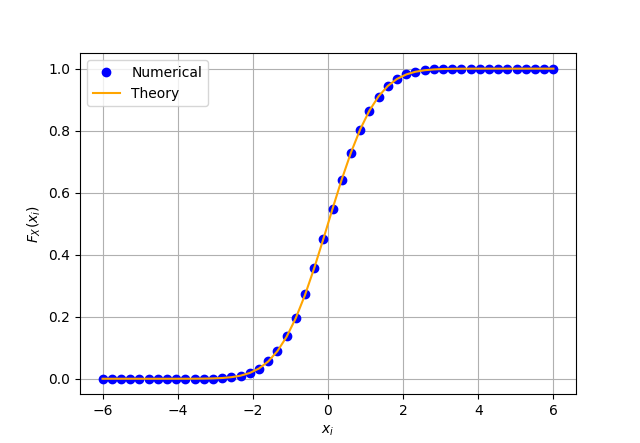
\includegraphics[width=\columnwidth]{./figs/2.2CDF.png}
\caption{The CDF of $X$}
\label{fig:2.2}
\end{figure}
Download the above file and execute the following command to produce Fig.\ref{fig:2.2}
\begin{lstlisting}
$ python3 2.2CDF.py
\end{lstlisting}
Some of the properties of CDF 
\begin{enumerate}
    \item $F_X(x)$ is non decreasing function.
    \item As $x \to -\infty$, $F_X(x) \to 0$ and when $x \to \infty$, $F_X(x) \to 1$
    \item Graph is linear upto some region around $x=0$.
\end{enumerate}

%%%%%%%%%%%%%%%%%%%%%%%%%%%%%%%%%%%%%%%%%%%%%
\item
Load gau.dat in python and plot the empirical PDF of $X$ using the samples in gau.dat. The PDF of $X$ is defined as
\begin{align}
p_{X}(x) = \frac{d}{dx}F_{X}(x)
\end{align}
What properties does the PDF have?
\\
\solution The PDF of $X$ is plotted in Fig. \ref{fig:2.3} using the code below
\begin{lstlisting}
https://github.com/bhargav0383/AI1110-Assignments/blob/main/RandomNumbers/codes/2.3PDF.py
\end{lstlisting}
Download the above files and execute the following commands to produce Fig.\ref{fig:2.3}
\begin{lstlisting}
$ python3 2.3PDF.py
\end{lstlisting}
\begin{figure}[!h]
\centering
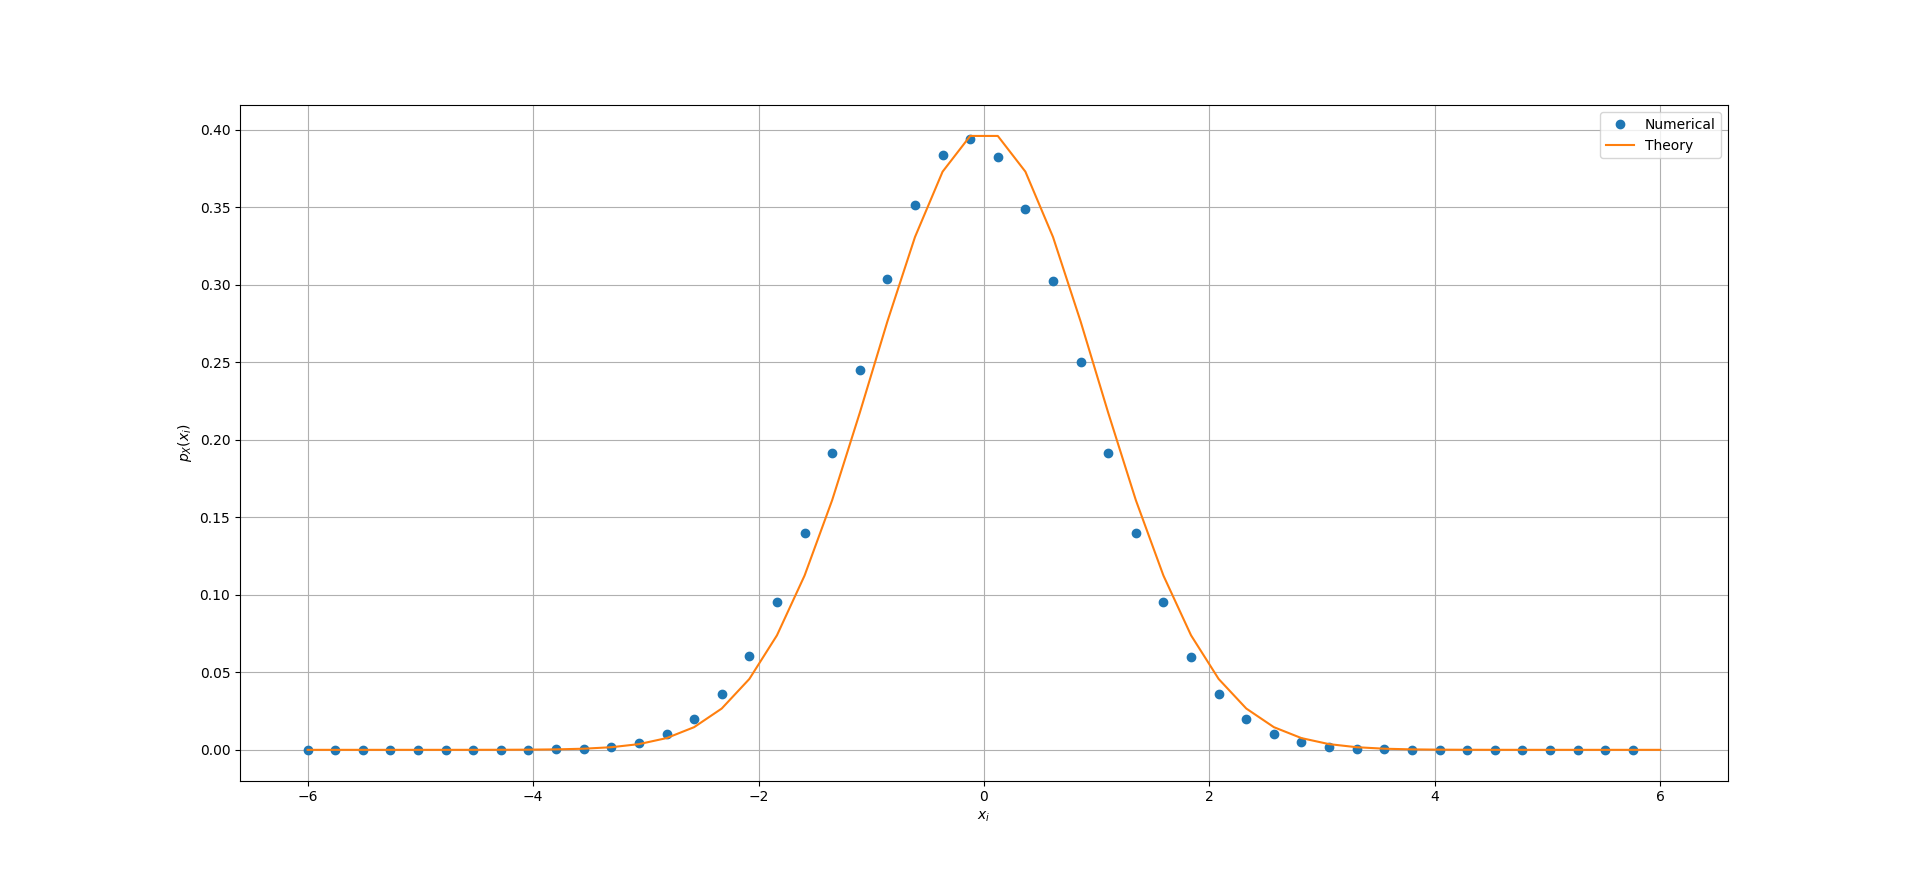
\includegraphics[width=\columnwidth]{./figs/2.3PDF.png}
\caption{The PDF of $X$}
\label{fig:2.3}
\end{figure}
Some of the properties of the PDF:
\begin{enumerate}
    \item Symmetric about $x=\mu$
    \item Area under the PDF graph is unity.
    \item Increasing function for $x<\mu$ and decreasing for $x>\mu$ and attains maximum at $x=\mu$.
\end{enumerate}
Let $x \sim \aleph(0,1)$. The Q-function $\displaystyle{Q(x)}$ is defined as:
\begin{align}
    \displaystyle{Q(x)} &= Pr\brak{X>x} \\
                        &= 1 - Pr\brak{X \leq x }\\
                        &= 1 - F_X(x) \\
                        &= 1 - \int_{-\infty}^{x}e^{-\frac{x^2}{2}}dx\\
                        % &= \frac{1}{2}\brak{\frac{2}{\sqrt{\pi}}\int_{x/\sqrt{2}}^{\infty}e^{-t^2}dt}\\
                        % &= \frac{1}{2}\brak{1-\frac{2}{\sqrt{\pi}}\int_{0}^{x/\sqrt{2}}e^{-t^2}dt}\\
                        % &= \frac{1}{2} - \frac{1}{2}\text{erf}\brak{\frac{x}{\sqrt{2}}}
\end{align}

%%%%%%%%%%%%%%%%%%%%%%%%%%%%%%%%%%%%%%%%%%%%%%%%%%%%%%%%%%%%%%%%%%%%%%%%%%%
\item Find the mean and variance of $X$ by writing a C program.\\
\solution Download the following files and execute the  C program.
\begin{lstlisting}
https://github.com/bhargav0383/AI1110-Assignments/blob/main/RandomNumbers/codes/2.4.c
https://github.com/bhargav0383/AI1110-Assignments/blob/main/RandomNumbers/codes/functions.h
\end{lstlisting}
Execute the above C program files using the following commands
\begin{lstlisting}
$ gcc 2.4.c
$ ./a.out
\end{lstlisting}
The actual analysis values,
\begin{align}
    \text{Mean}&= 0.000294 \\
    \text{Variance} &= 0.999561
\end{align}
%%%%%%%%%%%%%%%%%%%%%%%%%%%%%%%%%%%%%%%%%%%%%%%%%%%%%%%%%%%%
\item Given that 
\begin{align}
p_{X}(x) = \frac{1}{\sqrt{2\pi}}\exp\brak{-\frac{x^2}{2}}, -\infty < x < \infty,
\end{align}
repeat the above exercise theoretically.
\end{enumerate}
\solution 
CDF is defined as
    \begin{align}
        F_X(x)&=\int_{-\infty}^{\infty}p_X(x)dx\\
        \text{W.K.T,} \quad \boxed{F_X(x)=1}
    \end{align}
Mean is given by
    \begin{align}
        E(x)&=\int_{-\infty}^{\infty}xp_X(x)dx\\\
            &=\frac{1}{\sqrt{2\pi}}\int_{-\infty}^{\infty}x\exp\brak{-\frac{x^2}{2}}dx
    \end{align}
    It is a odd function function, So its value is 0.
    \begin{align}
        \boxed{E(x)=0}
    \end{align}
$E({x^2})$ is given by,
    \begin{align}
        E{(x^2)}&=\int_{-\infty}^{\infty}x^2p_X(x)dx \\
              &=\int_{-\infty}^{\infty}\frac{1}{\sqrt{2\pi}}x^2exp\brak{-\frac{x^2}{2}}dx \\
              &=\frac{1}{\sqrt{2\pi}}\brak{x\int x exp\brak{-\frac{x^2}{2}}dx}\\
              &-\frac{1}{\sqrt{2\pi}}\int \int \brak{x exp\brak{-\frac{x^2}{2}}}dx. dx\\
              &=\frac{1}{\sqrt{2\pi}}\int_{-\infty}^{\infty}exp\brak{-\frac{x^2}{2}}dx \\
              &=\frac{\sqrt{2\pi}}{\sqrt{2\pi}}\\&=1
    \end{align}
Variance is given by
    \begin{align}
        \text{var}\sbrak{U}=E(U^2)-(E(U))^2\\
        \therefore \boxed{\text{var}\sbrak{U}=1}
    \end{align}


%%%%%%%%%%%%%%%%%%%%%%%%%%%%%%%%%%%%%%%%%%%%%%%%%%%%%%%%%
\section{From Uniform to Other}
\begin{enumerate}[label=\thesection.\arabic*
,ref=\thesection.\theenumi]
%
\item
Generate samples of 
%
\begin{equation}
V = -2\ln\brak{1-U}
\end{equation}
%
and plot its CDF.  \\
\solution Download the following files and execute the  C program.
\begin{lstlisting}
https://github.com/bhargav0383/AI1110-Assignments/blob/main/RandomNumbers/codes/3.1.c
https://github.com/bhargav0383/AI1110-Assignments/blob/main/RandomNumbers/codes/functions.h
\end{lstlisting}
Execute the above C program files using the following commands
\begin{lstlisting}
$ gcc 3.1.c -lm
$ ./a.out
\end{lstlisting}
\begin{figure}[!h]
\centering
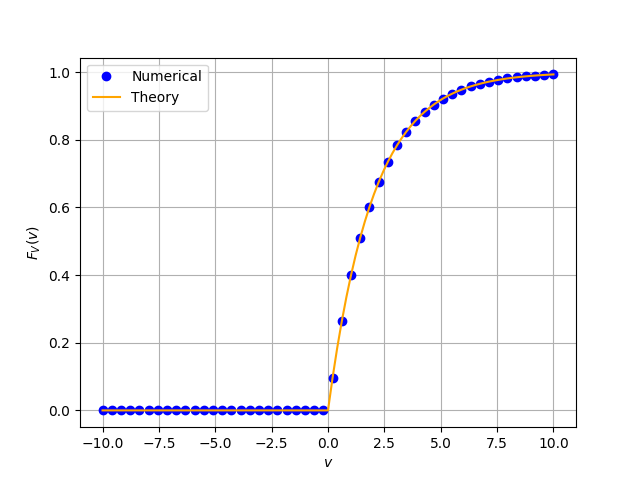
\includegraphics[width=\columnwidth]{./figs/3.1CDF.png}
\caption{The PDF of $X$}
\label{fig:3.1}
\end{figure}
The CDF of $V$ is plotted in Fig. \ref{fig:3.1} using the code below
\begin{lstlisting}
https://github.com/bhargav0383/AI1110-Assignments/blob/main/RandomNumbers/codes/3.1CDF.py
\end{lstlisting}
Download the above files and execute the following commands to produce plot Fig.\ref{fig:3.1}
\begin{lstlisting}
$ python3 3.1CDF.py
\end{lstlisting}

%%%%%%%%%%%%%%%%%%%%%%%%%%%%%%%%%%%%%%%%%%%%%%%%%%%%%%%%%%%%%5
\item Find a theoretical expression for $F_V(x)$.\\
\solution
If Y = g(X), 

W.K.T,
\begin{align}
  F_Y(y) = F_X(g^{-1}(y))  
\end{align}

\begin{align}
V &= -2\ln{(1-U)} \\
1-U &= e^{\frac{-V}{2}}\\
U &= 1 - e^{\frac{-V}{2}} \\ 
F_V(x) &= F_U(1 - e^{\frac{-x}{2}}) 
\end{align}
 \begin{align}
\implies
  F_V(x)=
  \begin{cases}
   0                         & x < 0 \\
	1 - e^{\frac{-x}{2}} & x \geq 0
	\end{cases}
 \end{align}
%\item
%Generate the Rayleigh distribution from Uniform. Verify your result through graphical plots.
\end{enumerate}

%%%%%%%%%%%%%%%%%%%%%%%%%%%%%%%%%%%%%%%%%%%%%%%%%%%%%%%%%%%%%%%%%%%%%
\section{Triangular Distribution}
\begin{enumerate}[label=\thesection.\arabic*
,ref=\thesection.\theenumi]
\item Generate
    \begin{align}
        T=U_1+U_2
    \end{align}
    \solution Download the following files and execute the  C program.
\begin{lstlisting}

\end{lstlisting}
Execute the above C program files using the following commands
\begin{lstlisting}

\end{lstlisting}

%%%%%%%%%%%%%%%%%%%%%%%%%%%%%%%%%%%%%%%%%%%%%%%%%%%%%%%%%%%%%%
\item Find the CDF of $T$.\\
\solution The CDF of $T$ is plotted in Fig. \ref{fig:4.2} using the code below
\begin{lstlisting}

\end{lstlisting}
Download the above files and execute the following commands to produce Fig.\ref{fig:4.2}
\begin{lstlisting}

\end{lstlisting}
% \begin{figure}[!h]
% \centering
% \includegraphics[width=\columnwidth]{./figs/4.5cdf.png}
% \caption{The CDF of $T$}
% \label{fig:4.2}
% \end{figure}

%%%%%%%%%%%%%%%%%%%%%%%%%%%%%%%%%%%%%%%%%%%%%%%%%%%%%%%
\item Find the PDF of $T$.\\
\solution The PDF of $T$ is plotted in Fig. \ref{fig:4.2} using the code below
\begin{lstlisting}

\end{lstlisting}
Download the above files and execute the following commands to produce Fig.\ref{fig:4.2}
\begin{lstlisting}

\end{lstlisting}
% \begin{figure}[!h]
% \centering
% \includegraphics[width=\columnwidth]{./figs/4.5pdf.png}
% \caption{The PDF of $T$}
% \label{fig:4.3}
% \end{figure}

%%%%%%%%%%%%%%%%%%%%%%%%%%%%%%%%%%%%%%%%%%%%%%%%%%%%%%%%%%%%%%%%%%%%%%%%
\item Find the Theoreotical Expression for the PDF and CDF of $T$\\
\solution
% \begin{align}
%     T&=U_1+U_2\\
%     \implies p_T(t)&=\int_{-\infty}^{t}p_{U1}(x)p_{U2}(y)dx\\
%     \text{As,}p_{U1}(x)&=p_{U1}(y)=p_{U}(u)\\
%     \implies p_T(t)&=\int_{-\infty}^{t}p_{U}(u)p_{U}(t-u)du
%     \end{align}
%     \begin{enumerate}
%         \item Theoretical PDF 
%         \begin{enumerate}
%             \item $t\le 1$
%             \begin{align}
%                 p_T(t)&=\int_{0}^{t}p_{U}(t-u)du\\
%                 \implies p_T(t)&=\int_{0}^{t} du=t
%             \end{align}
%             \item $t> 1$
%              \begin{align}
%                 p_T(t)&=\int_{0}^{1}p_{U}(t-u)du\\
%                 \implies p_T(t)&=\int_{t-1}^{1} du=2-t
%             \end{align}
%         \end{enumerate}
%         $\implies\boxed{ P_T(t) =
%         \begin{cases}
%          t     &0 \le t \le 1 \\
%          2-t   &1 < t \le 2\\
%          0     &t<0 \text{ or }t>2
%         \end{cases}
%         }$\\
%         \item Theoretical CDF 
%         \begin{align}
%             F_T(t)=\int_{-\infty}^{t}p_T(u)du
%         \end{align}
%         $\implies\boxed{
%             F_{T}(t)=
%             \begin{cases}
%              0   &t<0\\
%              \dfrac{t^2}{2} &0\le t \le 1\\
%              2t-1-\dfrac{t^2}{2} &1<t \le 2\\
%              1 &t>2
%             \end{cases}
%             }$\\
%     \end{enumerate}
    
%%%%%%%%%%%%%%%%%%%%%%%%%%%%%%%%%%%%%%%%%%%%%%%%%%%%%%%%55
\item Verify your results through a plot \\
\solution The Results are verfied in the plots
Fig \ref{fig:4.2} and Fig \ref{fig:4.3}
\end{enumerate}
\end{document}
